\begin{frame}[allowframebreaks]{LTI-Systeme in der realen Welt}

    Gibt es LTI-Systeme in der realen Welt?

    \framebreak

    \begin{figure}
        \centering
        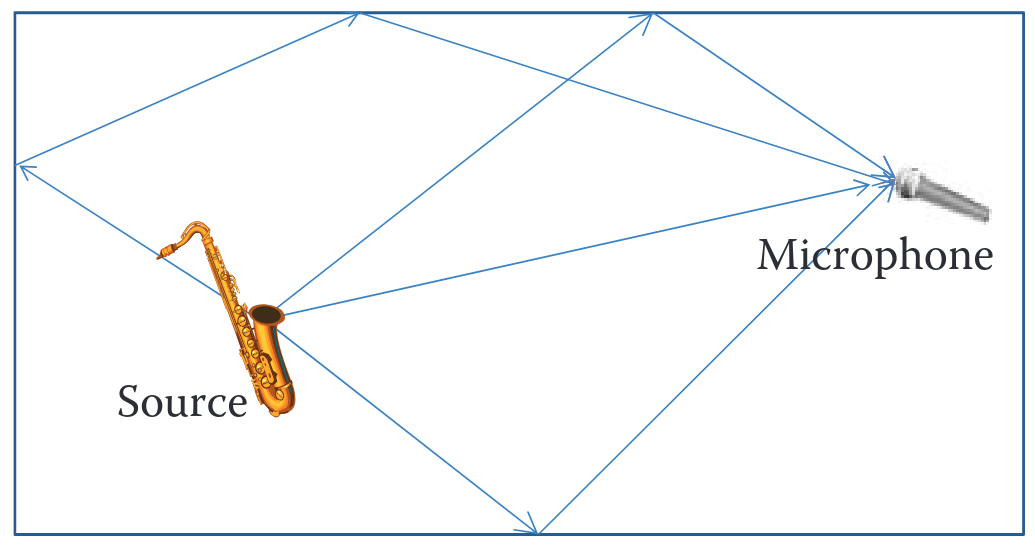
\includegraphics[width=0.8\textwidth]{Graphics/reiss_mcpherson_room_verb_diagram.png}
    \end{figure}\cite[Reiss, McPherson 2015]{reiss2015}

    \begin{figure}
        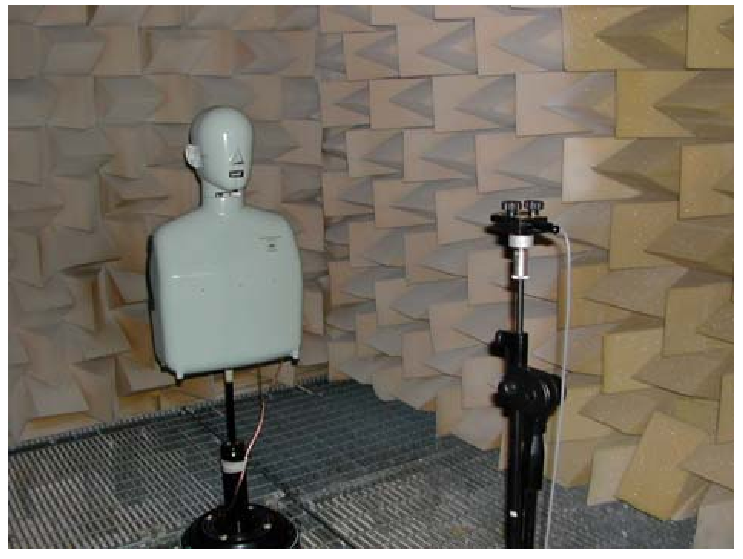
\includegraphics[width=0.6\textwidth]{Graphics/farina_anechoic.png}
    \end{figure} \cite[Farina 2007a]{farina2007a}
    
    \framebreak

    \begin{itemize}
        \item Räume
        \item Mikrofone
        \item Lautsprechersysteme (Speaker-Kabinetts für Gitarrenverstärker, Studiomonitore, Kopfhörer)
        \item noch viele mehr, über verschiedene Ingenieurswissenschaften verteilt
    \end{itemize}

    \framebreak

    Benötigt wird die Impulsantwort des Systems.
    \linebreak
    Beispiel Raumhall:
    \begin{itemize}
        \item Abspielen eines Impuls im Raum
        \item Aufnehmen des Raumschalls
    \end{itemize}

    \framebreak

    Aufnahme besteht aus Impuls, und der Transferfunktion des Raumes angewandt auf den Impuls.
    \linebreak
    \begin{itemize}
        \item Impulsantwort muss aus Aufnahme berechnet werden
        \item System nicht perfekt linear: Verstärker und Lautsprecher leicht nonlinear
        \item System nicht perfekt Zeit-invariant: Turbulenzen in Raumlauft verändern Schallgeschwindigkeit
    \end{itemize}
\end{frame}